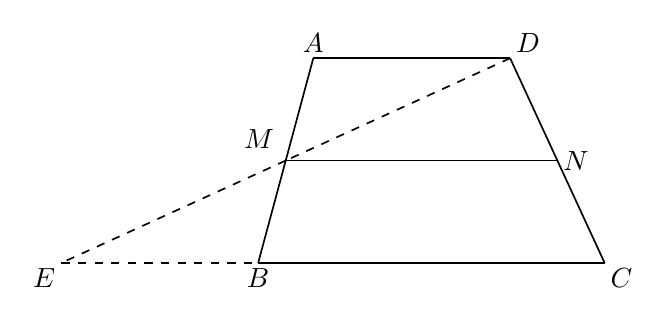
\begin{tikzpicture}[x=1cm,y=1cm,font=\normalsize,
 geometry edge/.style={solid,line width=.6pt},
 geometry mark/.style={solid,line width=.6pt},
 geometry label/.style={font=\normalsize,inner sep=2pt}]
\coordinate (A) at (1.5,2.6);
\coordinate (D) at (4,2.6);
\coordinate (B) at (0.8,0);
\coordinate (C) at (5.2,0);
\coordinate (M) at (1.15,1.3);
\coordinate (N) at (4.6,1.3);
\coordinate (E) at (-1.7,0);
\draw[geometry edge] (A)--(B);
\draw[geometry edge] (B)--(C);
\draw[geometry edge] (C)--(D);
\draw[geometry edge] (D)--(A);
\draw[geometry edge] (M)--(N);
\draw[geometry edge,dashed] (D)--(M);
\draw[geometry edge,dashed] (M)--(E);
\draw[geometry edge,dashed] (E)--(B);
\node[geometry label,above] at (A) {$A$};
\node[geometry label,above right] at (D) {$D$};
\node[geometry label,below] at (B) {$B$};
\node[geometry label,below right] at (C) {$C$};
\node[geometry label,above left,xshift=-2pt,yshift=2pt] at (M) {$M$};
\node[geometry label,right] at (N) {$N$};
\node[geometry label,below left] at (E) {$E$};
\end{tikzpicture}
